\documentclass[11pt]{article}
\usepackage[utf8]{inputenc}
\usepackage[margin=0.9in]{geometry}
\usepackage{natbib}
\usepackage{graphicx}
\usepackage{algorithm}
\usepackage{algorithmic}
\usepackage{amsmath}
\usepackage{amsfonts}
\usepackage{comment} 
\usepackage{appendix}
\usepackage{subfigure}
\usepackage[usenames,dvipsnames]{xcolor}
\usepackage{lipsum}  
\usepackage{tikz}


\usepackage{amsthm, amssymb}




% Nicer looking text, shorter
\usepackage{soul}
\usepackage{times}


\newcommand{\argmin}{\operatornamewithlimits{argmin}}
\newcommand{\argmax}{\operatornamewithlimits{argmax}}


\usepackage{color}
\definecolor{gray}{gray}{0.5}

\title{Coarsening graph networks which arise in the optimal design of robotic mechanisms}
\author{Aravind Baskar}
\date{}

\begin{document}

\maketitle

\section{Introduction}
Rigid-body mechanisms serve as useful building blocks for designing robotic systems such as legged robots. Graph networks arise from the solutions to optimal design problems of rigid-body mechanisms~[1,2]. These graphs are usually consisting of tens or hundreds of nodes which correspond to critical points, namely, saddle points, minima and maxima of a polynomial objective function. The edges represent gradient-descent paths from saddle points to the adjoining minima. Hence, saddle points exhibit two outgoing edges (degree two) while minima can have many incoming edges. A graph of this kind computed from such an optimal design problem is shown in Fig.~1. Each node of this graph is associated with a candidate design of robotic mechanisms, not shown here for lack of relevance to the course. The current project aims to use graph coarsening tools to condense these graphs for visualization and data presentation. An eigenvector based centrality measure is used for coarsening and hence the name spectral grouping. Via an algorithmic approach, following [3], that iterates over the nodes starting from the low ranked ones and moving higher up in the centrality measure, nodes exhibiting similar centrality measures are grouped together. This approach prioritizes nodes with high centrality measures over its neighbors to belong in a group of their own and hence, it retains key network topology. The graph can be further iterated in coarsening stages as desired till the whole graph collapses into a lone node. While an eigenvector centrality measure is used in this case, it is arguable that other metrics based on the physics of the underlying problem could be easily integrated into this coarsening framework.

\begin{figure}[htbp]
\centering
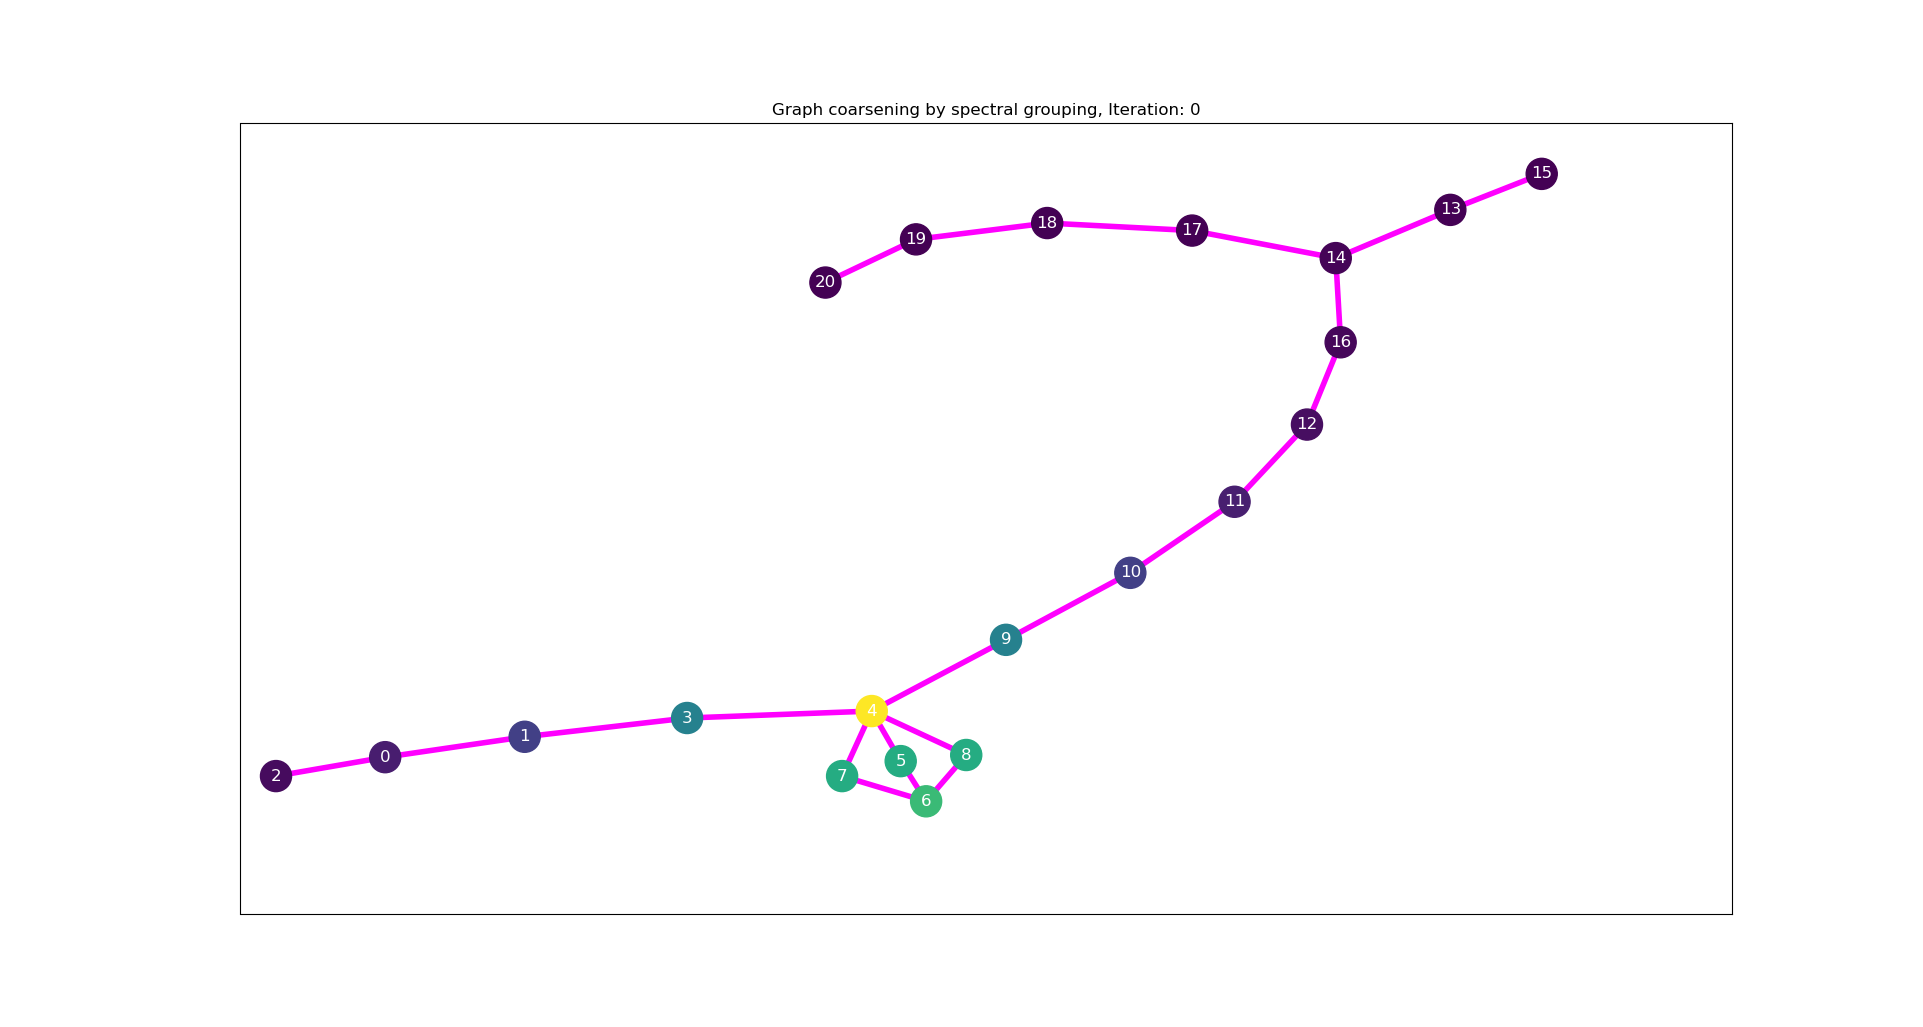
\includegraphics[width=1\textwidth]{Figure_0.png}
\caption{An example of a graph which arises in the design of robotic mechanisms. The nodes are color coded based on the eigenvector centrality measure.\label{fig:schematic}}
\end{figure}

\section{Methods and algorithms}

The vertex adjacency matrix~$A$ of an undirected graph~$G(V,E)$ is arrived based on computations not of great relevance to this project. The adjacency matrix is a square symmetric matrix consisting of zeros and ones where ones represent edges shared between the respective nodes. The components of the eigenvector corresponding to the largest eigenvalue is a good measure of the centrality of the nodes. This is a consequence of the \textbf{Perron-Forbenius} theorem which states that in real square matrices, there is a unique largest eigenvalue and its eigenvector can be written with strictly positive entries. The same measure is used by prominent search engines to rank order web-pages. Using power method, the eigenvector corresponding to the largest eigenvalue can be easily computed by repeated matrix product of a randomly chosen vector till convergence. Care must be taken to normalize the iteration result before furthering the iterations as the magnitude will increase if the largest eigenvector is of magnitude greater than 1.

Following this step, the algorithm described in~[3], namely, spectral grouping, is adopted for coarsening the graph in stages with some possible modifications. Based on the eigenvector centrality measure, the nodes are ranked from lowest to the highest. The nodes with higher centrality measures are key to the network connectivity and hence, it is desirable to group these as their own groups. This is prioritized by iterating the algorithm from the lowest centrality score to the highest and examining the neighbors in order. This algorithm groups neighboring nodes with the least difference in their centrality scores. If two or more neighboring nodes have the same centrality score, they are grouped in the same bin. Once a node is assigned to a group, it is skipped from the queue.

Finally, the new layout is generated for the coarsened graph by computing the centroid of the members of each group weighted by the eigen-centrality measure of the members of the group. This is a modification of the algorithm in~[3] where a simple centroidal rule was used. For the subsequent iteration, the diagonal of the modified adjacency matrix is updated with the number of nodes in each group to assign greater importance to groups with many nodes.

\section{Numerical section}
Using the method described above, the graph shown in Fig.~1 is coarsened in iterations as shown in Figs.~2-7. It may be seen that this algorithm prioritizes important nodes with high centrality to be their own groups. The layout is modified using the centroid of the nodes of each group weighted by the centrality measure of its members as mentioned. Note that there are several threshold and coarsening rules in the process flow that can be tweaked to slow or hasten the coarsening process. 

\begin{figure}[H]
\centering
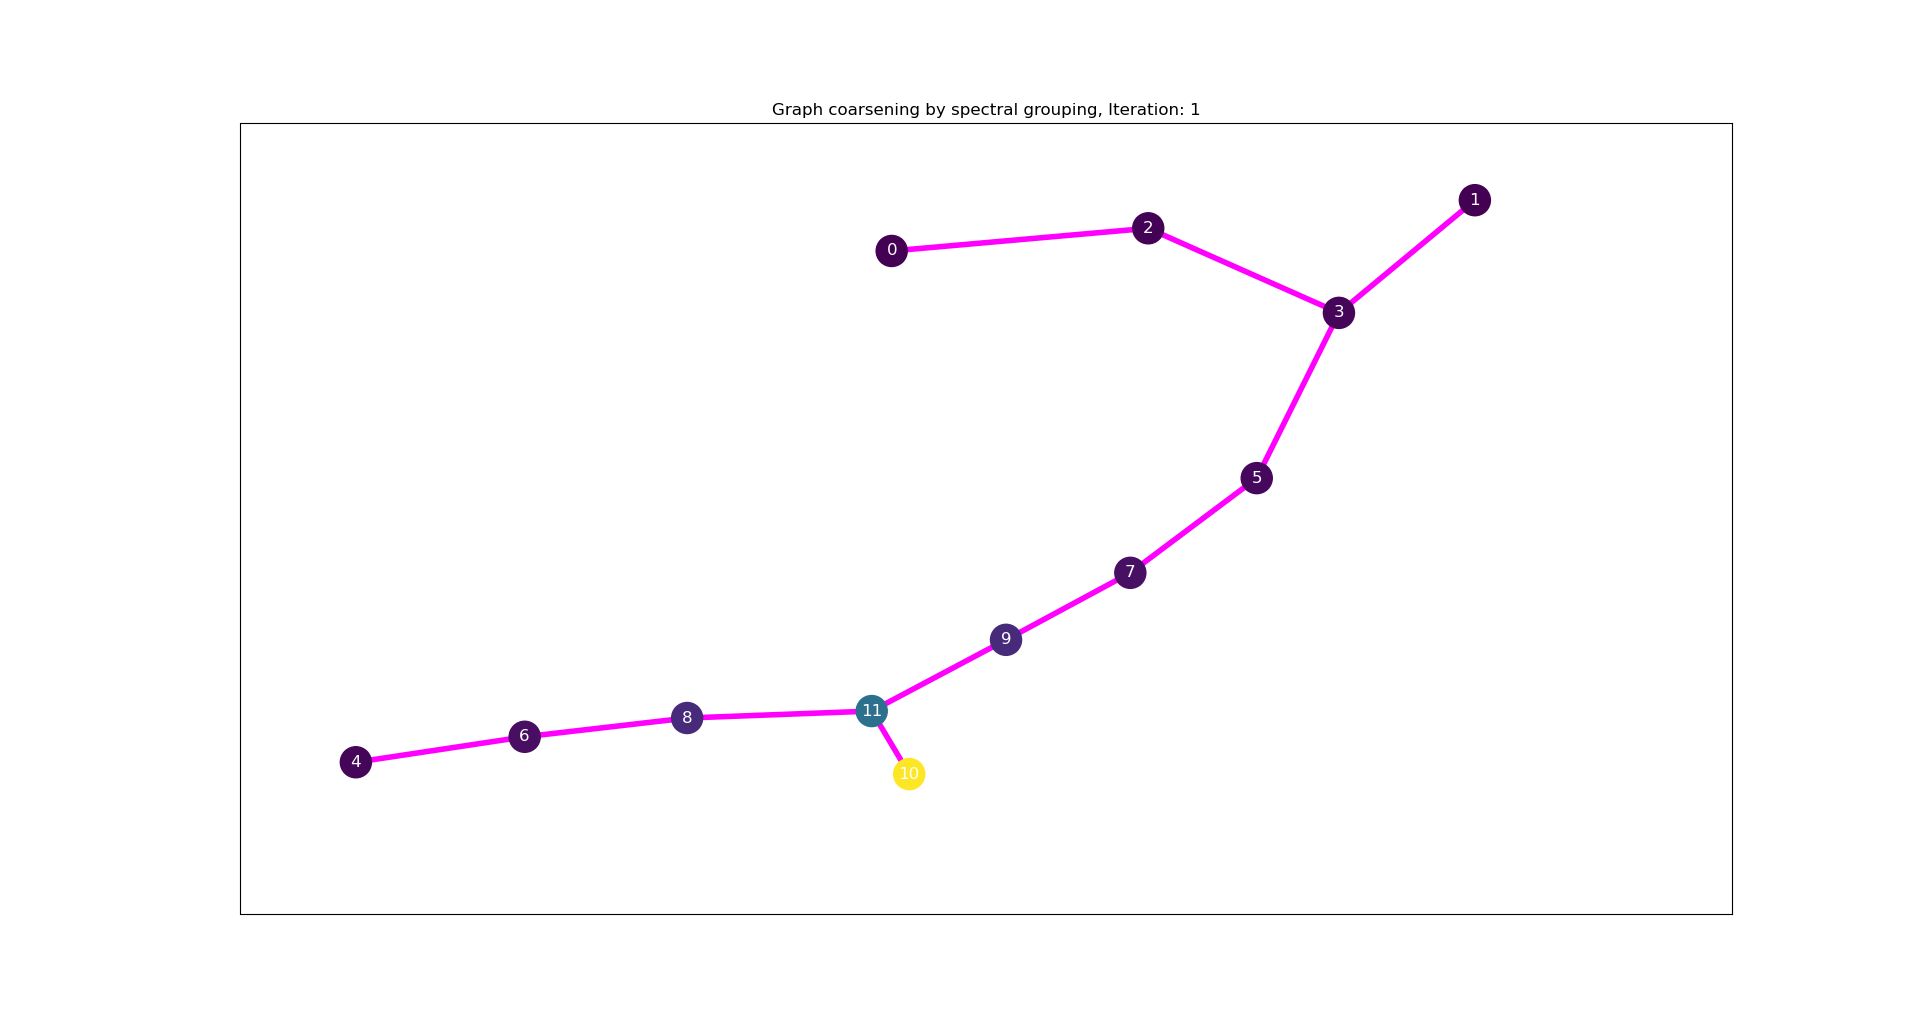
\includegraphics[width=1\textwidth]{Figure_1.png}
\caption{Graph coarsening Iteration 1: In the first iteration, the graph is coarsened from 21 nodes down to 12 nodes using spectral grouping. \label{fig:Iteration1}}
\end{figure}

\begin{figure}[H]
\centering
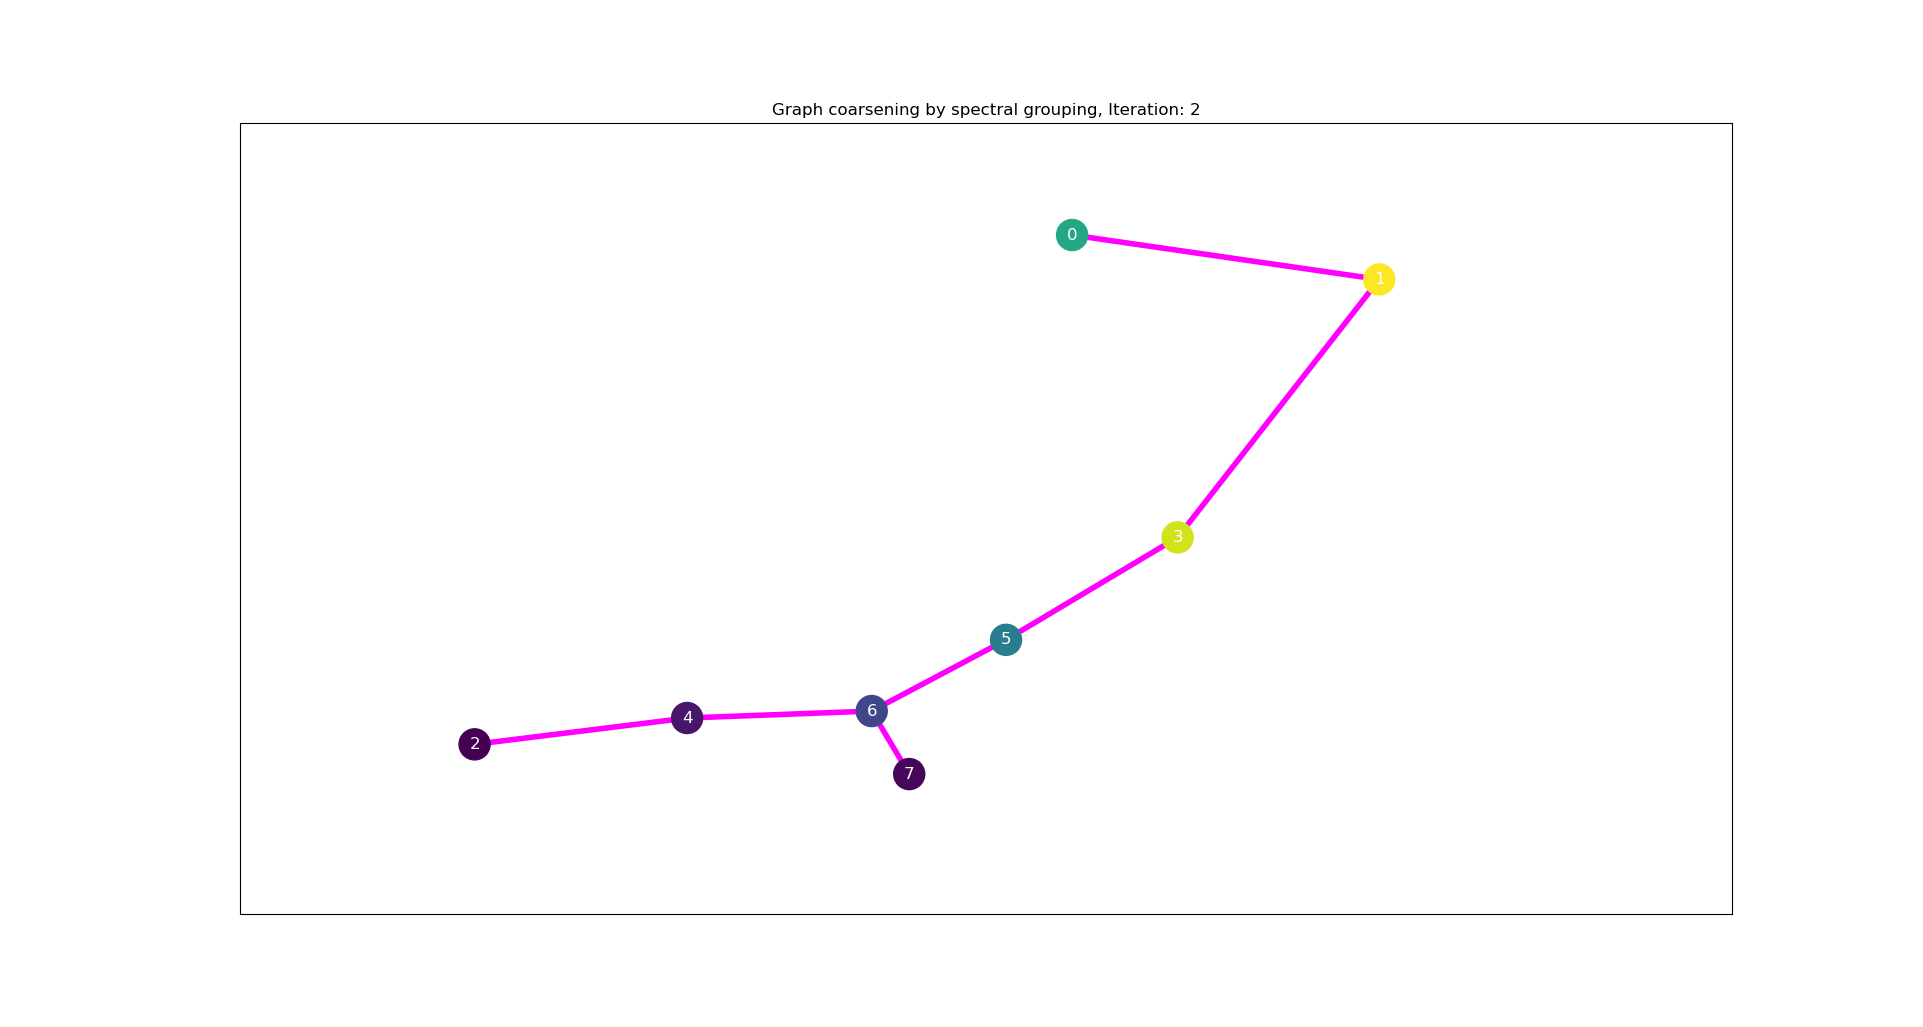
\includegraphics[width=1\textwidth]{Figure_2.png}
\caption{Graph coarsening Iteration 2: In the second iteration, the graph is coarsened from 12 nodes down to 8 nodes using spectral grouping as earlier.\label{fig:Iteration2}}
\end{figure}

\begin{figure}[H]
\centering
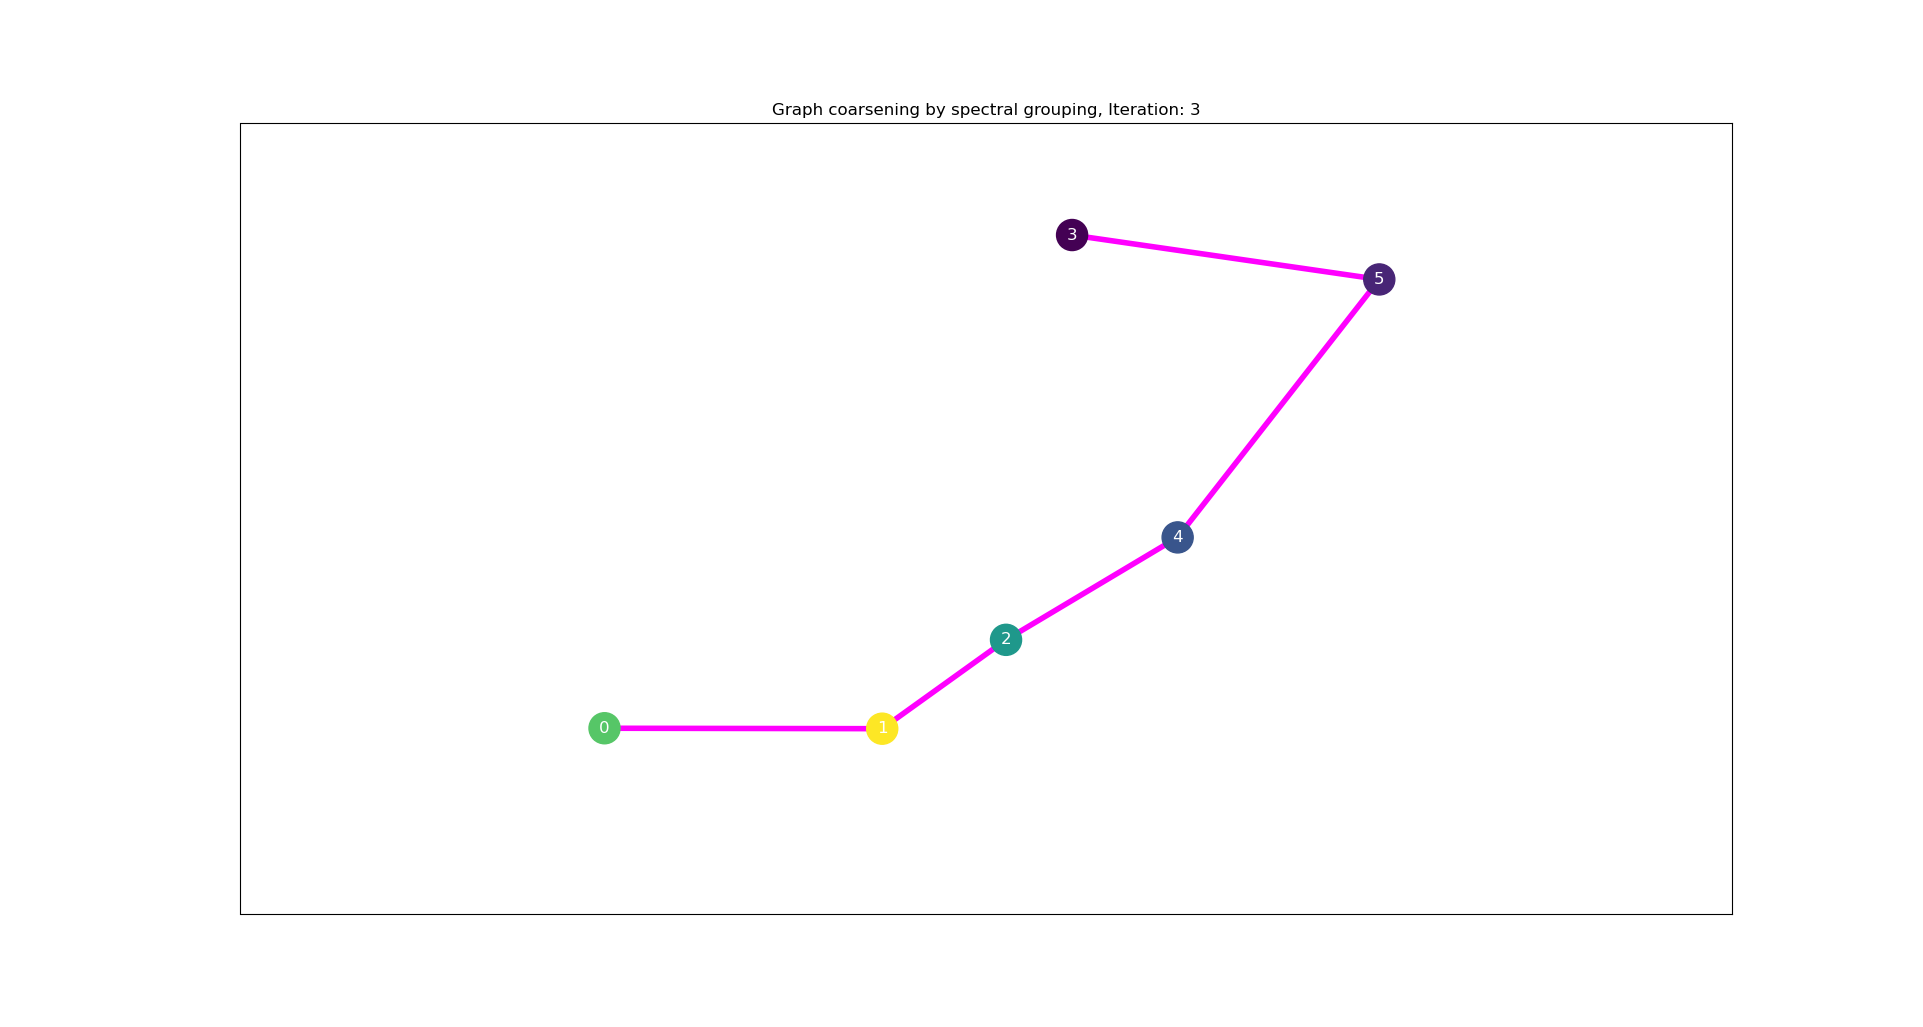
\includegraphics[width=1\textwidth]{Figure_3.png}
\caption{Graph coarsening Iteration 3: In the third iteration, the graph is coarsened from 8 nodes down to 6 nodes using spectral grouping.\label{fig:Iteration3}}
\end{figure}

\begin{figure}[H]
\centering
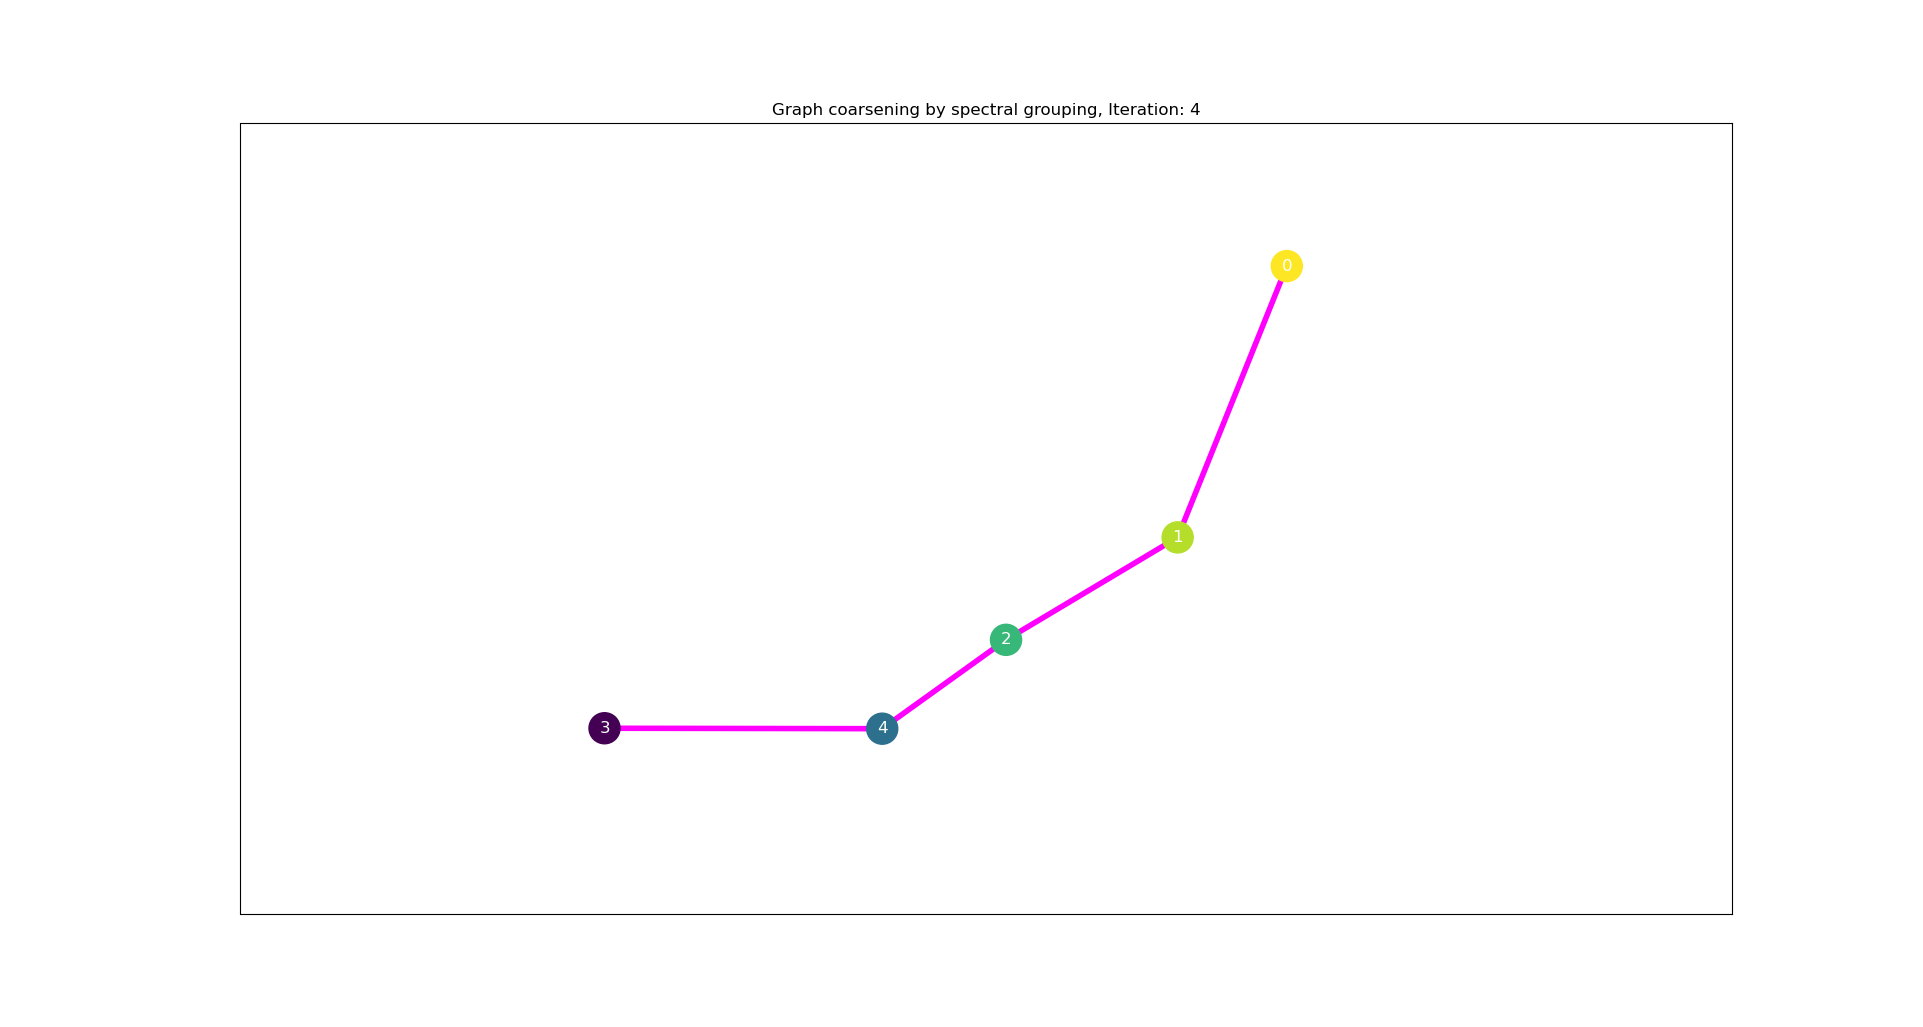
\includegraphics[width=1\textwidth]{Figure_4.png}
\caption{Graph coarsening Iteration 4: In the third iteration, the graph is coarsened from 6 nodes down to 5 nodes using spectral grouping.\label{fig:Iteration4}}
\end{figure}

\begin{figure}[H]
\centering
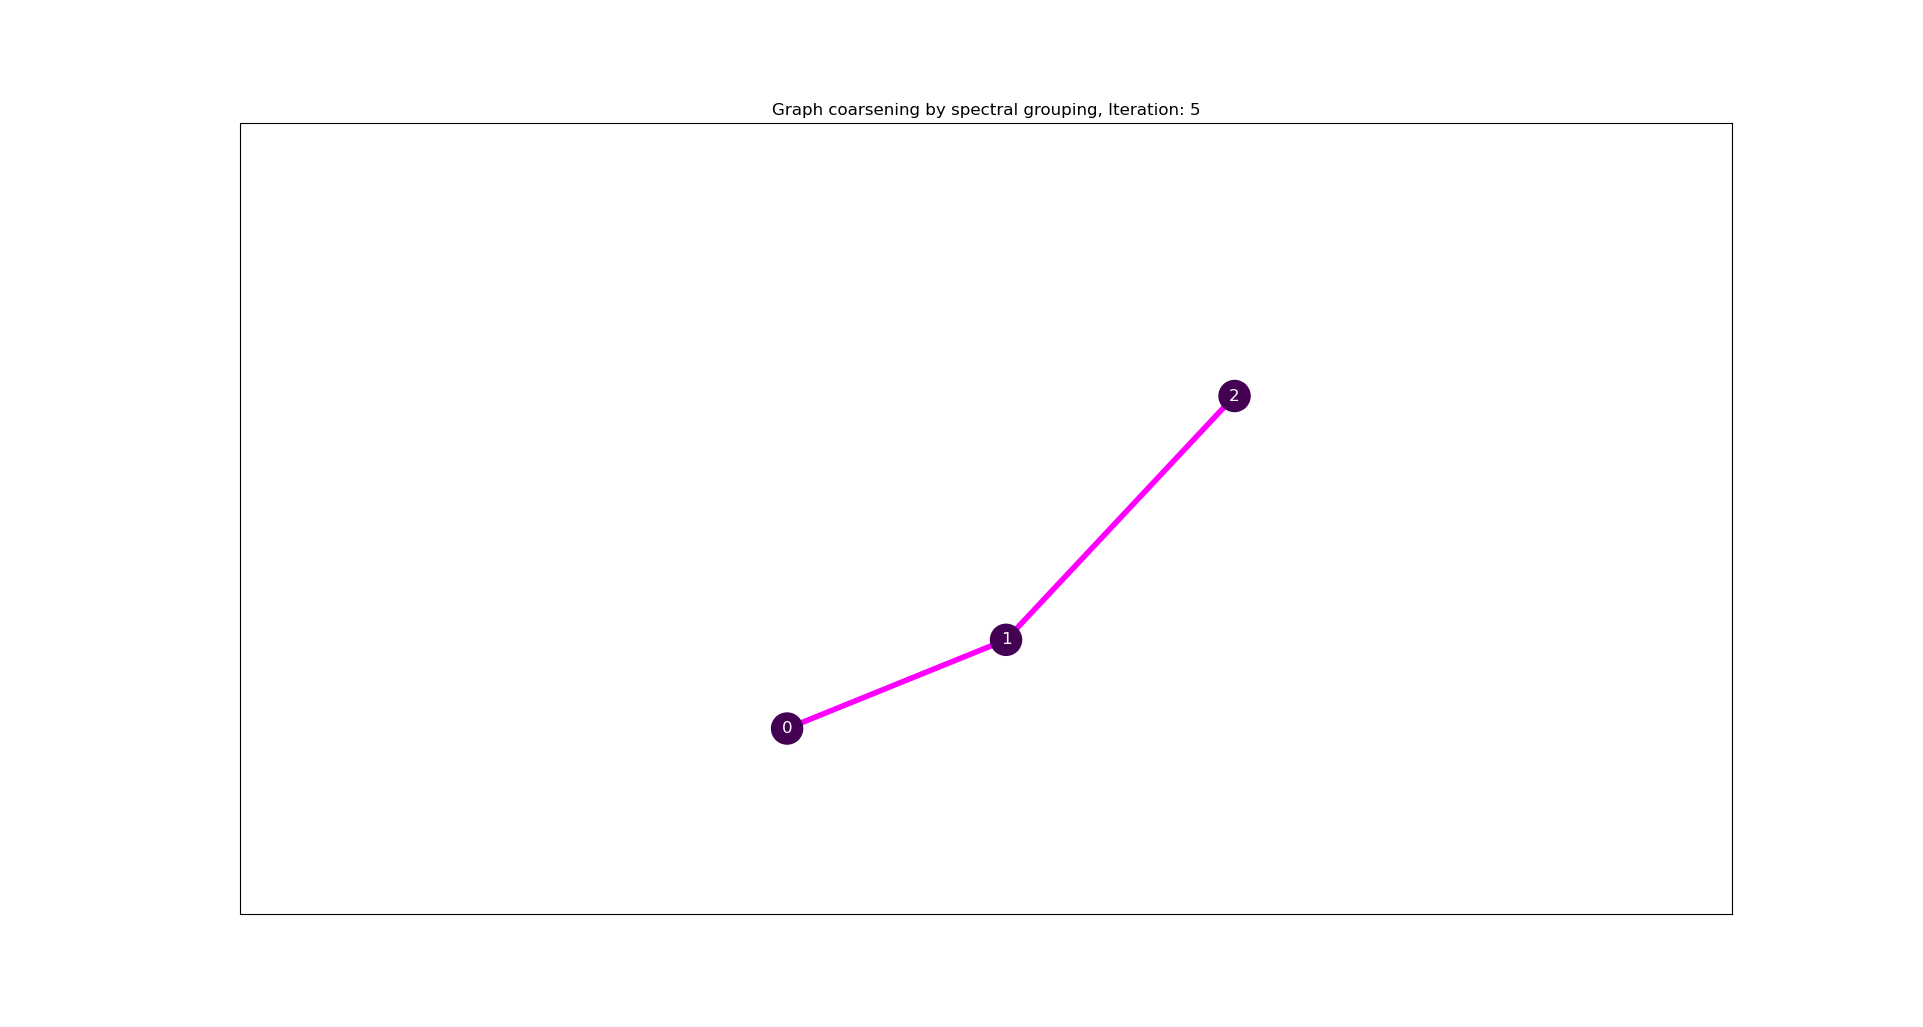
\includegraphics[width=1\textwidth]{Figure_5.png}
\caption{Graph coarsening Iteration 5: In the third iteration, the graph is coarsened from 5 nodes down to 3 nodes using spectral grouping.\label{fig:Iteration5}}
\end{figure}


\begin{figure}[H]
\centering
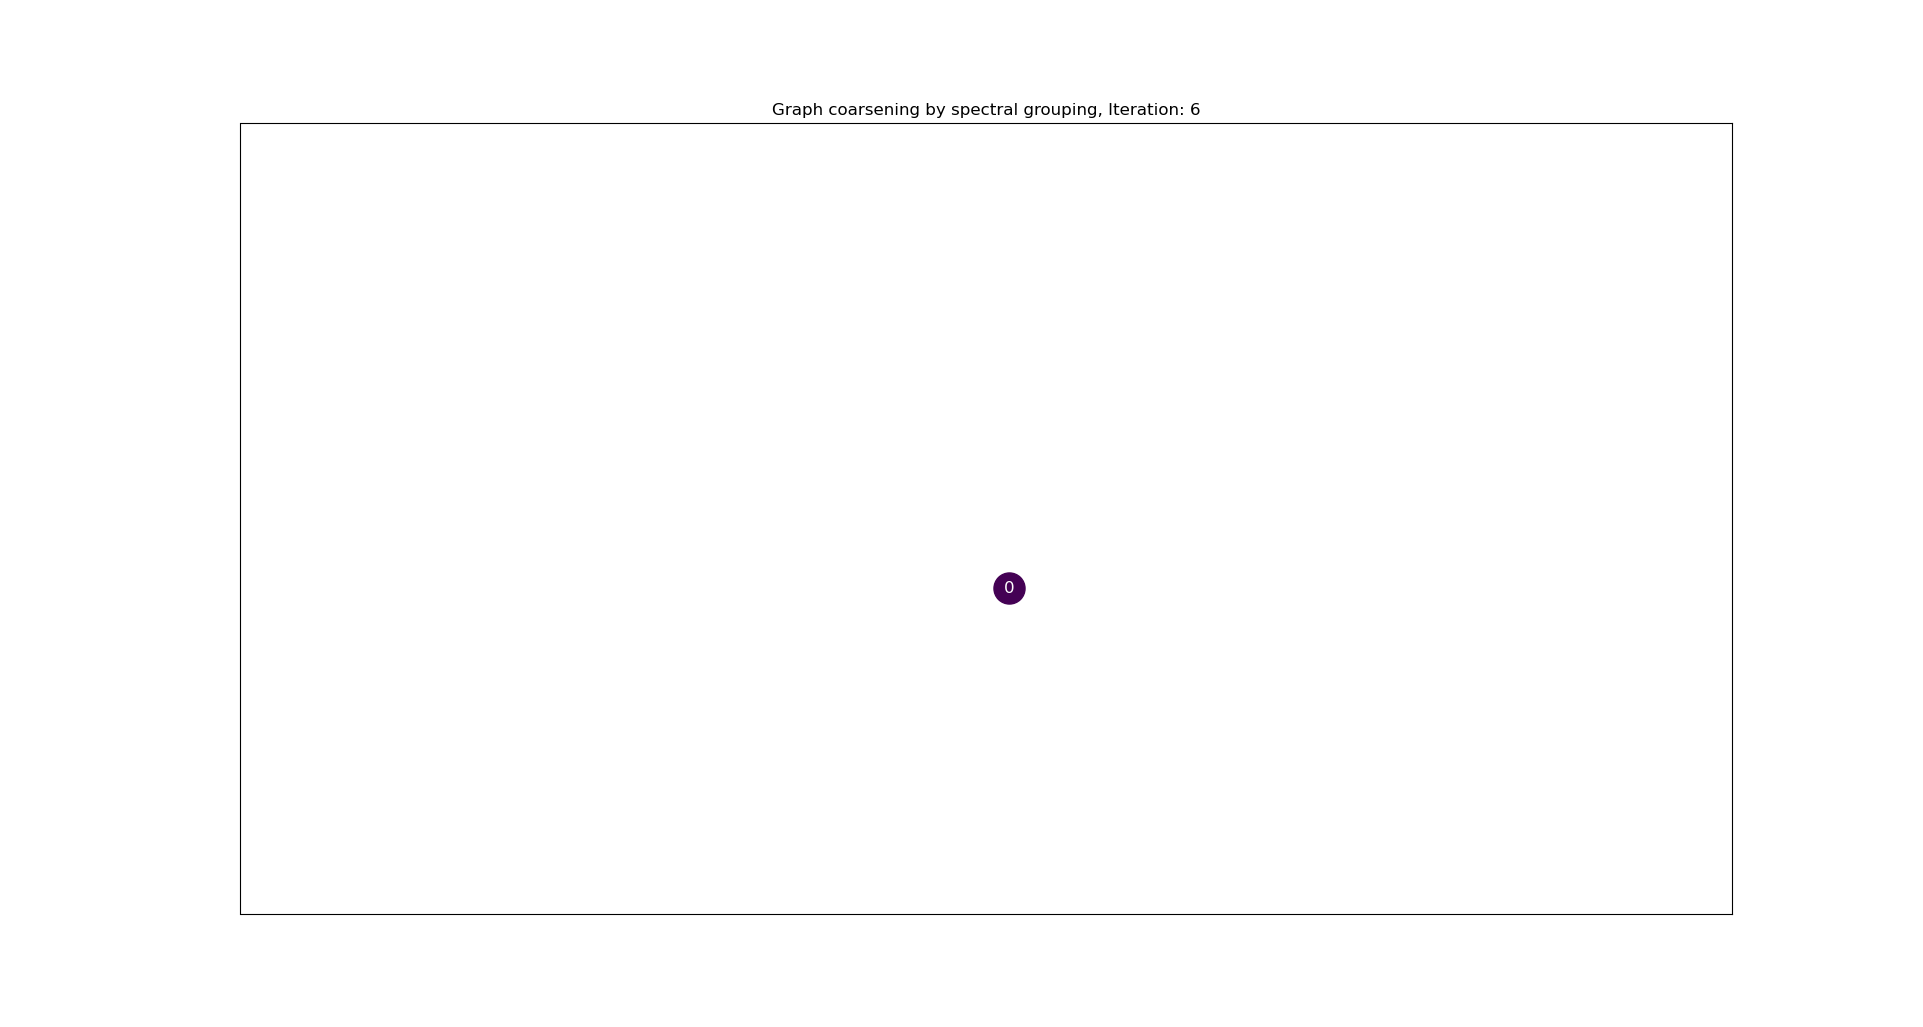
\includegraphics[width=1\textwidth]{Figure_6.png}
\caption{Graph coarsening Iteration 6: In the third iteration, the graph is coarsened from 3 nodes down to 1 node using spectral grouping.\label{fig:Iteration6}}
\end{figure}

\section{Conclusion}
In conclusion, this project was successful in implementing a graph coarsening scheme based on eigen-centrality measure found in recent literature with some slight modifications to customize the coarsening process. For presenting even larger graphs with hundreds of nodes, such graph coarsening schemes provide an elegant way to condense information. This project also aligns with the course objectives of understanding graph representation, analysis, feature extraction and node level clustering approaches on graphs.

\section*{References}
[1] Baskar, Aravind, Mark Plecnik, and Jonathan D. Hauenstein. "Computing saddle graphs via homotopy continuation for the approximate synthesis of mechanisms." Mechanism and Machine Theory 176 (2022): 104932.

\noindent
[2] Baskar, Aravind, Mark Plecnik, and Jonathan D. Hauenstein. "Finding Straight Line Generators Through the Approximate Synthesis of Symmetric Four-Bar Coupler Curves." In: Altuzarra, O., Kecskeméthy, A. (eds) Advances in Robot Kinematics (2022). Springer Proceedings in Advanced Robotics, vol 24. Springer, Cham.

\noindent
[3] Webb, Michael A., Jean-Yves Delannoy, and Juan J. De Pablo. "Graph-based approach to systematic molecular coarse-graining." Journal of chemical theory and computation 15.2 (2018): 1199-1208.

\end{document}